The first task is to classify players into one of two categories: significant contributors to the tournament, and non-significant contributors.  
This is because each team has more players than they usually will have play in the tournament, so we need only worry about players who actually will contribute to the tournament games.  
Whether or not someone was a significant contributor in any given game was determined by the percentage of possessions used during that game.  
If you were part of 10\% or less of total possessions, then you were not considered a significant contributor.  
Anything greater was considered a significant contribution to the game.  
The reason for 10\% is because there are multiple possible reasons a player could have some participation, but not actually be a significant contributor.  
For instance, if a game is going so well that the coach has no fear of losing, that coach may choose to put in players who, up to that point, had contributed nothing to the game so that they can have the experience of playing in the tournament.  
Alternatively, it's possible that a player started playing in the game, but before they managed to do very much became injured, and had to leave the game.  
Since there are 5 players on the court at a time, the 10\% threshold requires that, on average, you made some contribution to the game every other possession.  

Obviously, some of the statistics gathered have little to no bearing on whether or not a player will play in the tournament.  
For instance, no coach is going to keep you out of the game because you had 0 blocks, especially if you score 20 points on average per game.  
To determine which statistics were important and which were not, SKLearn's Lasso method was used on the averaged season statistics.  
The Lasso method utilizes L1 logistical regression for feature selection.  
Essentially, this amounts to weighting each statistic by how important it is in determining whether or not they will be significant contributors in the tournament while trying to keep the total weights as small as possible.  
Nonzero weights correspond to features that were important for classification, and zero coefficients those that could be ignored.  
\begin{figure}
\centering
\caption{Variable weights from Lasso Method (weights of 0 excluded)}
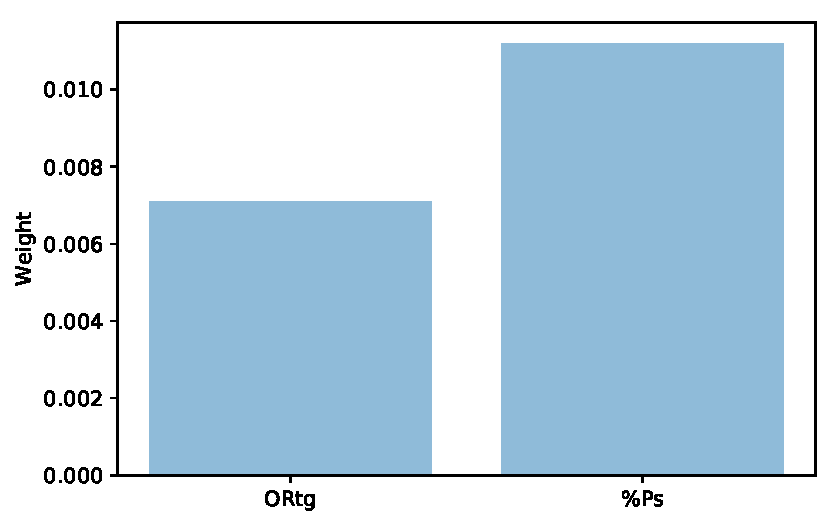
\includegraphics[width=0.5\textwidth]{../Feature_Weights.pdf}
\label{fig:weights1}
\end{figure}
The only variables with nonzero coefficients were Offensive Rating (ORtg) and Percent of Possessions Used (\%Ps), as shown in Figure \ref{fig:weights1}.  
Utilizing these two variables alone achieved 87.89\% accuracy \footnote{Data from 2013-2016 was used for training with 2017 data used for testing.} in determining which players would contribute to the tournament and which would not.  
If, for one reason or another, the algorithm predicted that fewer than five players would contribute, everyone was used instead, since you can't have less than five players for a game.  